\documentclass[border=10pt]{standalone}
\usepackage{tikz}
\usetikzlibrary{arrows.meta, calc}

\begin{document}
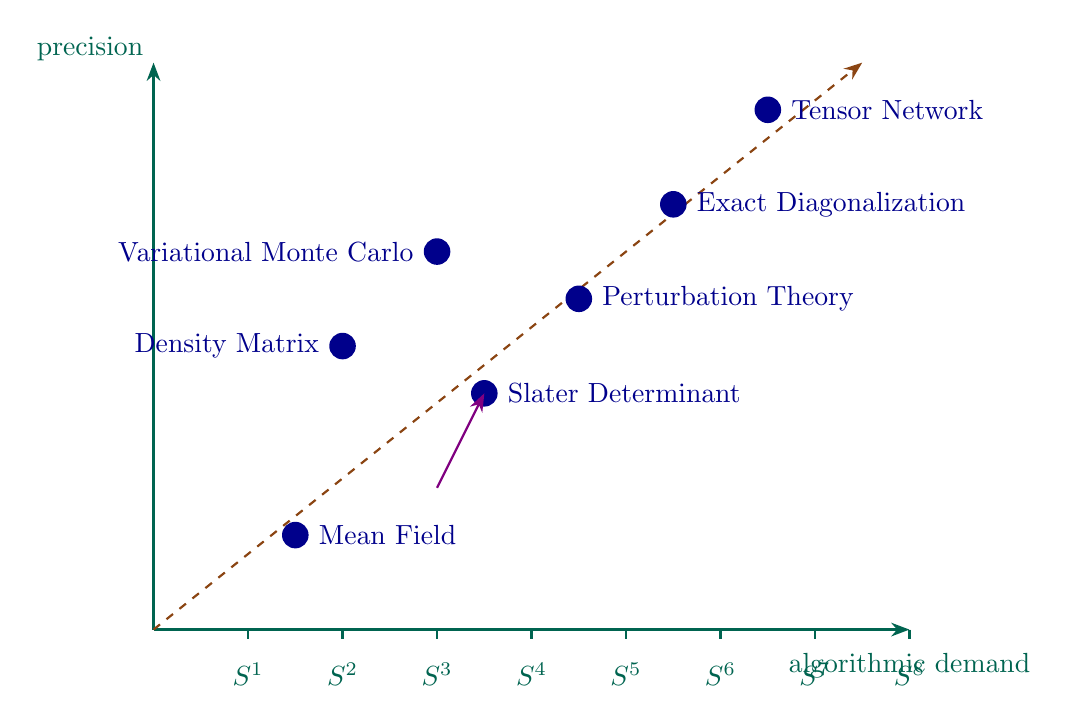
\begin{tikzpicture}[scale=1.2, >=Stealth]

% Define colors
\definecolor{teal}{RGB}{0, 100, 80}
\definecolor{blue}{RGB}{0, 0, 139}
\definecolor{brown}{RGB}{139, 69, 19}
\definecolor{purple}{RGB}{128, 0, 128}

% Axes
\draw[teal, thick, ->] (0,0) -- (0,6) node[anchor=east, yshift=5pt] {precision};
\draw[teal, thick, ->] (0,0) -- (8,0) node[anchor=north, yshift=-5pt] {algorithmic demand};

% Tick marks and labels on x-axis
\foreach \i in {1,2,...,8} {
    \draw[teal, thick] (\i,0) -- (\i,-0.1) node[anchor=north, yshift=-5pt] {$S^{\i}$};
}

% Dashed trend line
\draw[brown, thick, dashed, ->] (0,0) -- (7.5,6);

% Data points and labels
\coordinate (MF) at (1.5,1.0);
\coordinate (SD) at (3.5,2.5);
\coordinate (PT) at (4.5,3.5);
\coordinate (ED) at (5.5,4.5);
\coordinate (TN) at (6.5,5.5);
\coordinate (VMC) at (3.0,4.0);
\coordinate (DM) at (2.0,3.0);

% Draw points
\foreach \point in {MF, SD, PT, ED, TN, VMC, DM} {
    \fill[blue] (\point) circle (4pt);
}

% Labels
\node[blue, anchor=west, xshift=5pt] at (MF) {Mean Field};
\node[blue, anchor=west, xshift=5pt] at (SD) {Slater Determinant};
\node[blue, anchor=west, xshift=5pt] at (PT) {Perturbation Theory};
\node[blue, anchor=west, xshift=5pt] at (ED) {Exact Diagonalization};
\node[blue, anchor=west, xshift=5pt] at (TN) {Tensor Network};
\node[blue, anchor=east, xshift=-5pt] at (VMC) {Variational Monte Carlo};
\node[blue, anchor=east, xshift=-5pt] at (DM) {Density Matrix};

% Purple arrow pointing to Slater Determinant
\draw[purple, thick, ->] (3.0,1.5) -- (SD);

\end{tikzpicture}
\end{document}